\documentclass[thesis.tex]{subfiles}

\begin{document}
\chapter{Background and Related Work}
The field of neuroinformatics, despite its recent emergence, has burgeoned rather rapidly, has produced and adopted a wide variety of techniques that can be used for performing white matter integrity and structure research. Since my work has greatly relied on the ideas and methods used in CoBundleMAP and within the FBA, in this chapter an overview of these approaches will be given, together with my reflections on this particular topic.

%=======================================================================================================
\section{Diffusion weighted MRI}
%------------------------------------------------------------------------------------
\subsection{General information}
Diffusion weighted imaging (DWI) is a well-established, noninvasive method of acquiring information about the structure of biological tissues. It is based on the fact that in unrestricted mediums water movement is absolutely random (Brownian movement), while restricted areas force molecules to diffuse in specific directions. These two possibilities are called isotropic diffusion and anisotropic diffusion respectively. Diffusion weighted MRI is capable of measuring the amount of such water motion along any chosen axis. To define the direction of the diffusion in three-dimensional space, observations are made by applying diffusion gradient pulses along several non-collinear orientations \cite{ChanraudDTI}.
Anisotropic water diffusion inside of biological tissue is explained as the result of molecular movement being restricted by specific barriers such as cell membranes or axon fibres \cite{diffusion1990Moseley}. Specifically in the brain white matter fiber tracts, that consist of axon bundles, the presence of myelination forces water to diffuse preferentially along axonal fiber directions \cite{WMdiffusion} \cite{Mori1999DiffusionMR}. Existence of such dominant direction is the basis for a wide variety of techniques. Based on diffusion tensor analysis, white matter tractography and calculation of various characteristic metrics can be executed \cite{Basser1995InferringMF}. Among such measures are Fractional Anisotropy, Mean Diffusivity, Axial Diffusivity and Radial Diffusivity, all of which are used in existing implementation of CoBundleMap pipeline, and will be discussed further in more details.

DWI allows us to perform a noninvasive analysis of the micro-structure of tissue, which is extremely useful in cases of white matter research, where possibility of in vivo investigation is of significant value. DWI has significantly contributed to our understanding of the human brain. The possibility to examine the white matter bundle structures and, when present, find pathological abnormalities has helped us comprehend various neurological diseases and disorders \cite{dwiDiseases, ChanraudDTI, dtiGeneralGood}, as well as effects of aging on human brain \cite{moseleyAging} and mechanisms of neuroplasticity \cite{Tournier2004FODdeconv, dwiDiseases}.

%------------------------------------------------------------------------------------
\subsection{Diffusion tensor imaging}
Diffusion Tensor Imaging (DTI) is a quantitative imaging method that provides the possibility to infer brain micro-structure properties based on data acquired through DWI \cite{BasserHow}. Common uses of the DTI include: white matter fiber tractography, brain connectivity analysis, and assessment of parameters that describe integrity and general state of both white and grey matter.

% \begin{figure}
% \centering
% 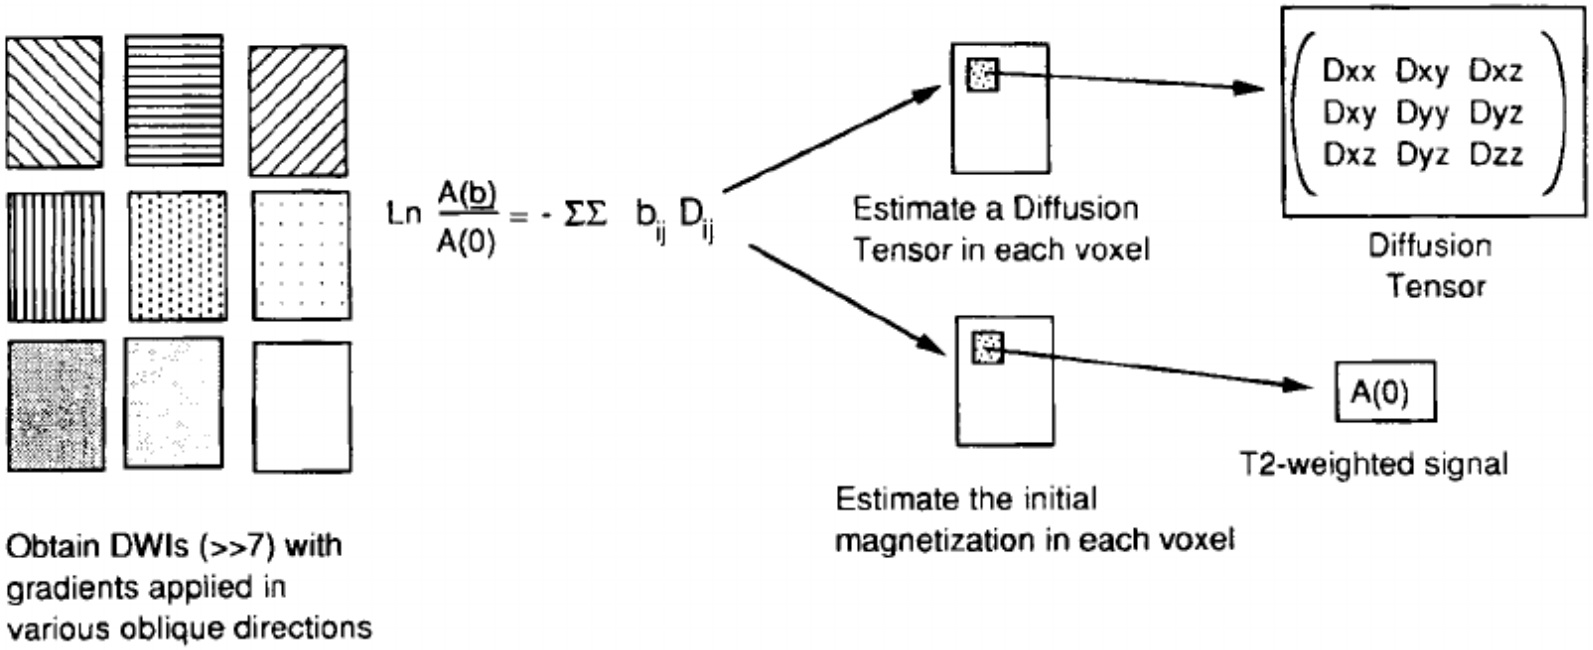
\includegraphics[width=14cm,height=14cm,keepaspectratio]{thesis_radomskyi/images/dti-scheme-cite-Basser1995InferringMF.png}
% \caption{\textbf{DTI Scheme.} This scheme depicts the basic steps involved in diffusion tensor imaging approach. The output of DTI for each processed voxel is a 3x3 diffusion tensor and a $T_2$-weighted scalar A(0) \cite{Basser1995InferringMF}.}
% \label{fig:dti-scheme}
% \end{figure}


The main idea of this approach lies in estimating a symmetric and positive definite tensor $D_{eff}$ -- effective diffusion tensor, within each voxel. This is performed by selecting a local orthogonal coordinate system and calculating three corresponding diffusion coefficients in these directions \cite{Basser1994DTI}. The diffusion tensor, being a symmetric 3 $\times$ 3 matrix, can be described by three positive eigenvalues ($\lambda_1, \lambda_2, \lambda_3$) and three orthogonal eigenvectors ($e_1, e_2, e_3$). These eigenvalues represent the magnitude of diffusion within each given voxel, while eigenvectors reflect the corresponding directions. Such tensor may be interpreted as a mathematical representation of three-dimensional ellipsoid \cite{Basser1995InferringMF}, describing diffusion characteristics in individual voxels (Figure \ref{fig:dti-scheme}).

\begin{figure}
\centering
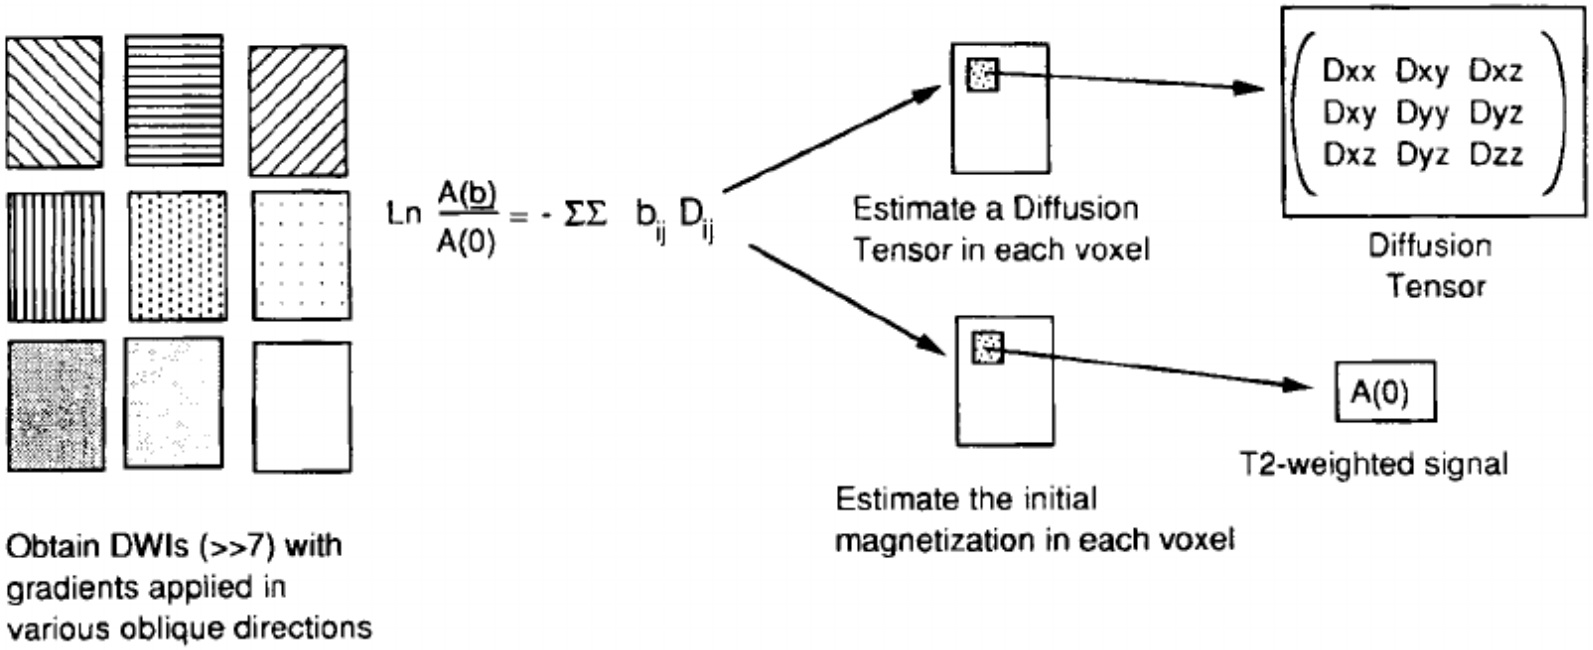
\includegraphics[width=14cm,height=14cm,keepaspectratio]{thesis_radomskyi/images/dti-scheme-cite-Basser1995InferringMF.png}
\caption{\textbf{DTI Scheme.}}
\label{fig:dti-scheme}
\end{figure}

From the parameters that are contained in DT, a set of scalar quantities that measure fundamental features of diffusion within tissues can be extracted  \cite{Basser1995InferringMF, Basser1996FA}.

The most basic of such metrics is eigenvalue average, or trace of DT, referred to as Mean Diffusivity (MD). It is rotationally invariant and reflects the magnitude of overall diffusion within the voxel:
\[ MD = \frac{tr(D)}{3} = \frac{\lambda_1 + \lambda_2 + \lambda_3}{3} \]
Higher values of MD are indicators of isotropic diffusion (possible axon degeneration or demyelination), while lower MD is primarily observed in regions of anisotropic diffusion (high myelination, dense axonal packing). Another rotationally invariant measure extracted from TD is FA. It describes the degree of orientational preference within a voxel, or in other words, amount of anisotropy, and is often used as a measure of white matter integrity. In relation to DT eigenvalues, it defines the extent to which one eigenvalue prevails over other two and is computed based on MD:
\[ FA = \sqrt{\frac{(\lambda_1 - MD)^2 + (\lambda_2 - MD)^2 + (\lambda_3 - MD)^2}{2(\lambda_{1}^2 + \lambda_{2}^2 + \lambda_{3}^2)}} \]

Existing implementation of CoBundleMAP also performs computation of two more DT-derived metrics related to analysis of white matter pathologies \cite{dtiGeneralGood} -- Axial Diffusivity (AD) and Radial Diffusivity (RD). AD reflects axonal integrity and \cite{RDmyelination} equals to the value of the largest eigenvalue:
\[AD = \lambda_1\]
while RD is defined by secondary eigenvalues and reflect myelin integrity \cite{RDmyelination}:
\[RD = \frac{\lambda_2 + \lambda_3}{2}\]
Though it is worth mentioning that interpretation of AD and RD should be performed with care and preferably in combination with other DTI-derived features \cite{rd-ad-crit}.
Nevertheless, analysis of diffusion measures and their correlations is a reliable method of gaining valuable insights about the condition of white matter tissue. For example, simultaneous rise in FA combined with lower RD is a sign of dense axonal packing or high myelination, while the mirrored case -- low FA and high RD are signals of either axonal degeneration or demyelination \cite{fa-fd-correlation}.
%------------------------------------------------------------------------------------
\subsection{Voxel based analysis}

Voxel-based analysis (VBA) is a technique used for voxel-wise analysis of diffusion images across a given population of subjects, capable of identifying local differences and correlations in the structure of brain tissue. It is an important and well-established approach, permitting comparison of the voxels between the same areas of different brains, which in case of significant differences can reveal the presence of a degenerative disease. The essential principle on which VBA is based, is retrieval of anatomical correspondences between the subjects by spatially normalizing images to s a common stereotactic space (usually a brain atlas), using image registration algorithms \cite{vbaMechelli}. Image registration commonly consists of two distinct steps, which sequentially increase similarity between the input and reference images. First one is computation of the linear transformation, including estimation of the rigid-body transformation, used for rotation and translation of the image, followed by global scaling and skewing. This allows to perform correction of differences in the brain size across the population as well as revision of possible orientation variations. Second step accounts for global nonlinear differences and involves estimation of the coefficients of the basis function, minimizing the residual sum of squared differences between them and simultaneously maximizing the smoothness of the deformation \cite{vbaAshburner}. Deformation field, derived from image registration, contains information about adjustments made for matching voxels of the input image and the template. One of the important outcomes of the image spatial normalization, is that exact voxel-wise volume fluctuations can be computed from extracted deformation fields as Jacobian determinants. Analysis of Jacobian determinants as well as the deformation fields themselves establishes what is known as tensor-based morphometry or deformation-based morphometry \cite{vbaKurth}.

\subsection{Constrained spherical deconvolution}
Spherical deconvolution is an approach used for estimations of the fiber orientation distribution (FOD) function within the voxels of diffusion-weighted images. Introduction of this approach allowed to perform identification of multiple fiber orientations within a single voxel, as shown on Figure \ref{fig:sd-is-good}. It is based on several assumptions about the nature of diffusion inside white matter tissue and implies that it is possible to approximate the measured diffusion-weighted signal as a sum of the signals emitted by each of the orientationally distinct fiber population that is present in the sample \cite{csd1TOURNIER}. Therefore, the signal measured from a single fiber population is expressed as a symmetric response function $R(\theta)$, where $\theta$ is elevation angle in spherical coordinates, while the signal originating from multiple incoherently aligned populations is defined as a sum of such functions, aligned with respect to their orientation (via azimuthal angle $\phi$ in spherical coordinates) and weighted by the share of volume ($f_{i}$), that each population occupies within the voxel \cite{csd1TOURNIER}: \[S(\theta, \phi) = \sum_{i}f_{i}A_{i}R(\theta)\]
Here, $A_{i}$ is an operator of rotation onto direction ($\theta_{i}, \phi_{i}$). The signal can be then subsequently interpreted as a convolution over spherical coordinates of the FOD function and response function:
\[S(\theta, \phi) = F(\theta, \phi) \otimes R(\theta)\]
FOD estimation can then be seen as a problem of inferring the distribution from the measured signal, given a suitable response function \cite{csdDellAcqua2019}. Constrained spherical deconvolution (CSD) is a further development of these ideas. The main improvement of CSD over simple spherical deconvolution is the introduction of a non-negativity constraint on the values in the computed FOD, leading to elimination of the noise caused by high angular frequencies \cite{dwi2fod2-csd}.

\begin{figure}
\centering
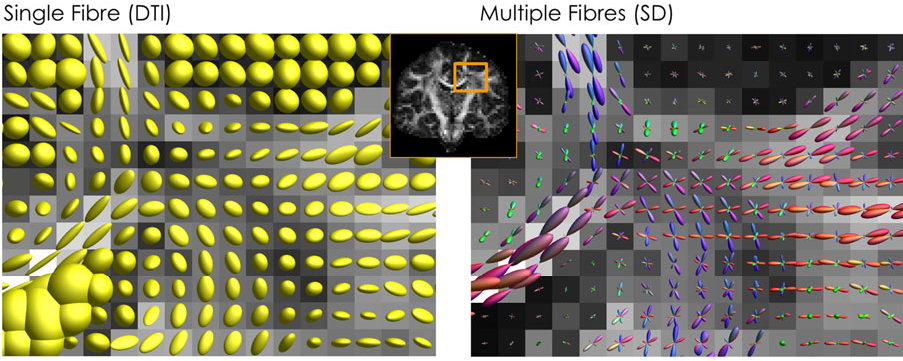
\includegraphics[width=14cm,keepaspectratio]{thesis_radomskyi/images/sd-is-good.png}
\caption{\textbf{Comparison of DTI and SD.} Diffusion tensor (left) is capable of describing the average diffusion profile in each image voxel, thus capturing only dominant fiber population. Spherical deconvolution (right), on the other hand, is capable of identifying multiple populations. \cite{csdDellAcqua2019}.}
\label{fig:sd-is-good}
\end{figure}

%=======================================================================================================
\section{Fixel based analysis}
Although VBA of diffusion MRI, namely analysis of tensor-derived FA values, is a rather common approach to researching structure of white matter in the brain, it has some restrictions. Since FA, as well as other diffusion measures, is computed as a value averaged within the whole voxel, it doesn't account for the fact that most white matter voxels (around 90\% as reported in \cite{crossingFibers2013}) contain several crossing fibres. Inside such voxels FA is affected by all fiber populations that are present, thus producing values which do not reliably represent any underlying tract. Figure \ref{fig:percent-of-non-dominant-volume-fraction} shows statistics of affected white matter voxels and degree of their contamination with non-dominant fibre orientations.
This could not only affect precision of the whole system, but also prevents us from a more robust and specific analysis of individual fibres.
A possible solution for this problem could be utilization of diffusion MRI mixture models, which are able to recognise multiple fibre populations within a single voxel. A common name for such a fibre population is \textit{fixel} \cite{aboutFixels2015Raffelt}, while commodity of methods that are using this approach is called Fixel-based analysis (FBA). In this section I will make an overview of papers introducing fixel-based approach to white matter analysis, as well new metrics for measuring nervous fibre integrity, density and thickness.

\begin{figure}
\centering
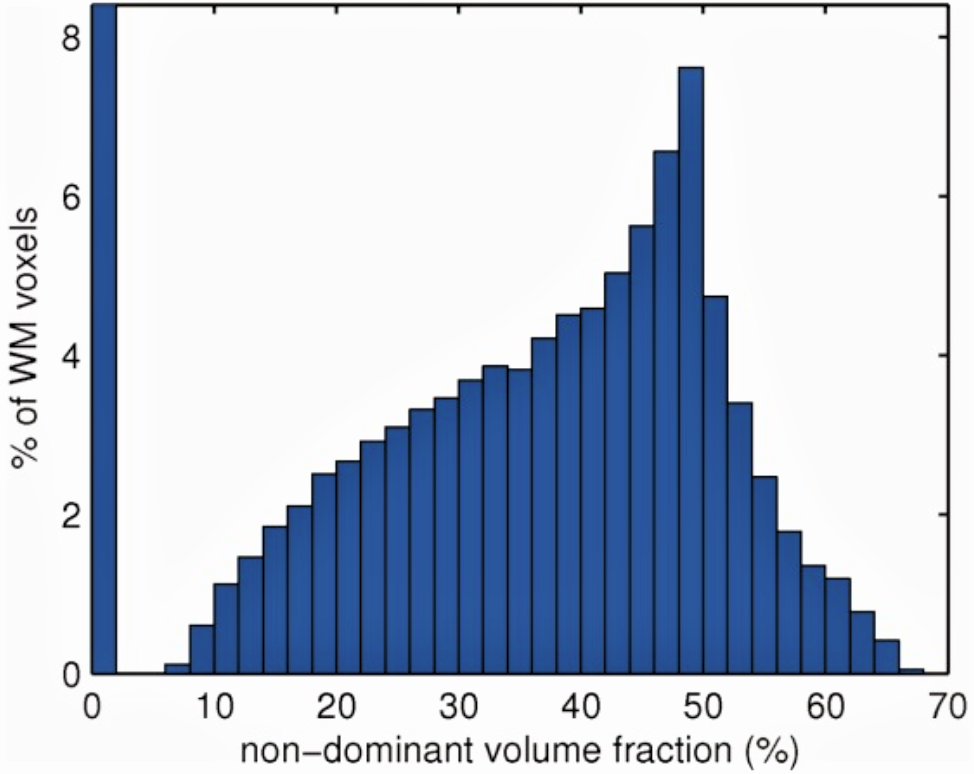
\includegraphics[width=10cm,height=10cm,keepaspectratio]{thesis_radomskyi/images/percent-of-non-dominant-volume-fraction-cite-crossingFibers2013.png}
\caption{\textbf{Non-dominant Volume Fraction of White Matter Voxels} Histogram depicting non-dominant volume fraction measured by CSD over all white matter voxels \cite{crossingFibers2013}}
\label{fig:percent-of-non-dominant-volume-fraction}
\end{figure}

\subsection{Fiber density and cross-section}
Investigation of white matter tissue is closely related to estimation of its integrity, ability to connect different regions of the brain and transfer information. The extent to which separate bundles contribute to such connectivity may be characterised by the total number of axons within the bundle, their thickness and degree of myelination. One of the proposed metrics, that is capable of measuring these properties of white matter tracts is Apparent Fiber Density (AFD) \cite{afd2012Raffelt}. This metric introduces a novel approach to computation of fiber-specific parameters, allowing to perform analysis of individual fiber populations in voxels that contain multiple tracks, by leveraging the information, obtained within image spatial normalization process. The important development of this approach is Fiber density cross-section (FDC) metric \cite{fdcAndFBA2017Raffelt}. This method further improves the ideas of AFD and defines FDC as a measure of white matter integrity, consisting of two related values -- Fiber density (FD), which is basically AFD, and Fiber cross-section (FC), which describes local volumetric differences within the examined population. Both metrics, similar to AFD, are based on information, contained within deformation fields which are produced by image registration. In addition to allowing computation of fiber-specific parameters, approach adopted within FBA also allows to derive better insights about the structure and integrity of the tissue. As can be observed from the Figure \ref{fig:difference-fd-fc-fdc}, new metrics allow to distinguish between different types of intra-axonal volume changes, providing important information for deeper analysis of underlying causes.

\begin{figure}
\centering
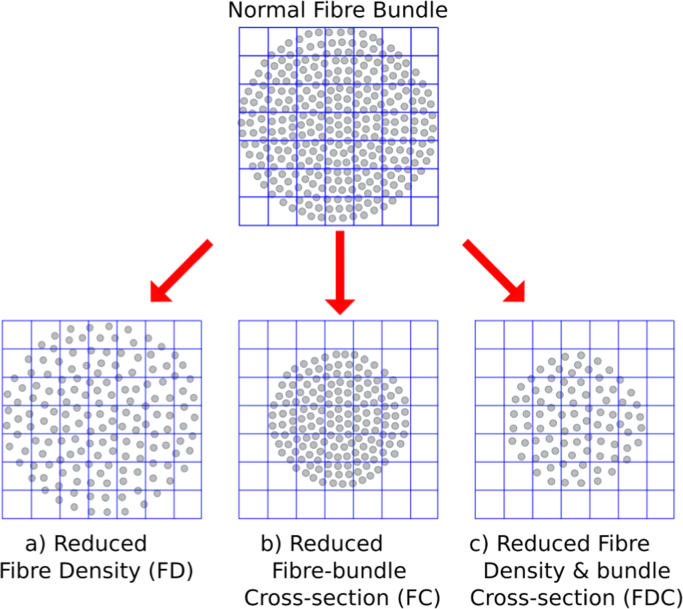
\includegraphics[width=10cm,height=10cm,keepaspectratio]{thesis_radomskyi/images/difference-fd-fc-fdc.jpg}
\caption{\textbf{Different types of intra-axonal volume reduction} By performing analysis of both FC and FD values we may achieve better insights about underlying causes\cite{fdcAndFBA2017Raffelt}}
\label{fig:difference-fd-fc-fdc}
\end{figure}




\section{CoBundleMAP}
Since the main objective of this work is to further extend CoBundleMAP, it is essential to understand its inner mechanisms and the principles upon which it is built. BundleMAP and CoBundleMAP are dMRI image processing tools, developed within the Department of Computer Science, University of Bonn. Results obtained through these pipelines contain, among other things, feature vectors that can be further utilized in machine learning and data processing algorithms, or used for visual analysis of specific white matter areas. Following subsections contain a short overview of steps performed and algorithms used within the scope of CoBundleMAP pipeline. Since CoBundleMAP is an improved, two-dimensional manifestation of BundleMAP, I will start with the overview of ideas implemented in the latter.

\subsection{BundleMAP overview}
BundleMAP tries to solve the problem of deriving features, which are specific for an interpretive evaluation of different degenerative white matter diseases, as well as performing research of the tissue structure. The main principle of BundleMAP is to combine joint parametrization and manifold learning for extracting bundle-specific duffusivity measures \cite{Khatami2017BundleMap}. Joint parametrization can be described as a process of finding anatomical correspondences between specific brain regions among given population of patients. If we know such unambiguous areas, we can perform localised comparisons between subjects and find areas of interest for each given application case. Features that are extracted contain such diffusion measures as FA, MD, RD and AD.


The pipeline can be logically split into four distinct steps (Figure \ref{fig:bundlemap-steps}): fiber tractography, followed by supervised and unsupervised outlier removal, manifold learning, and feature extraction. Next subsections contain more specific information and explanations about each performed step.

\begin{figure}
\centering
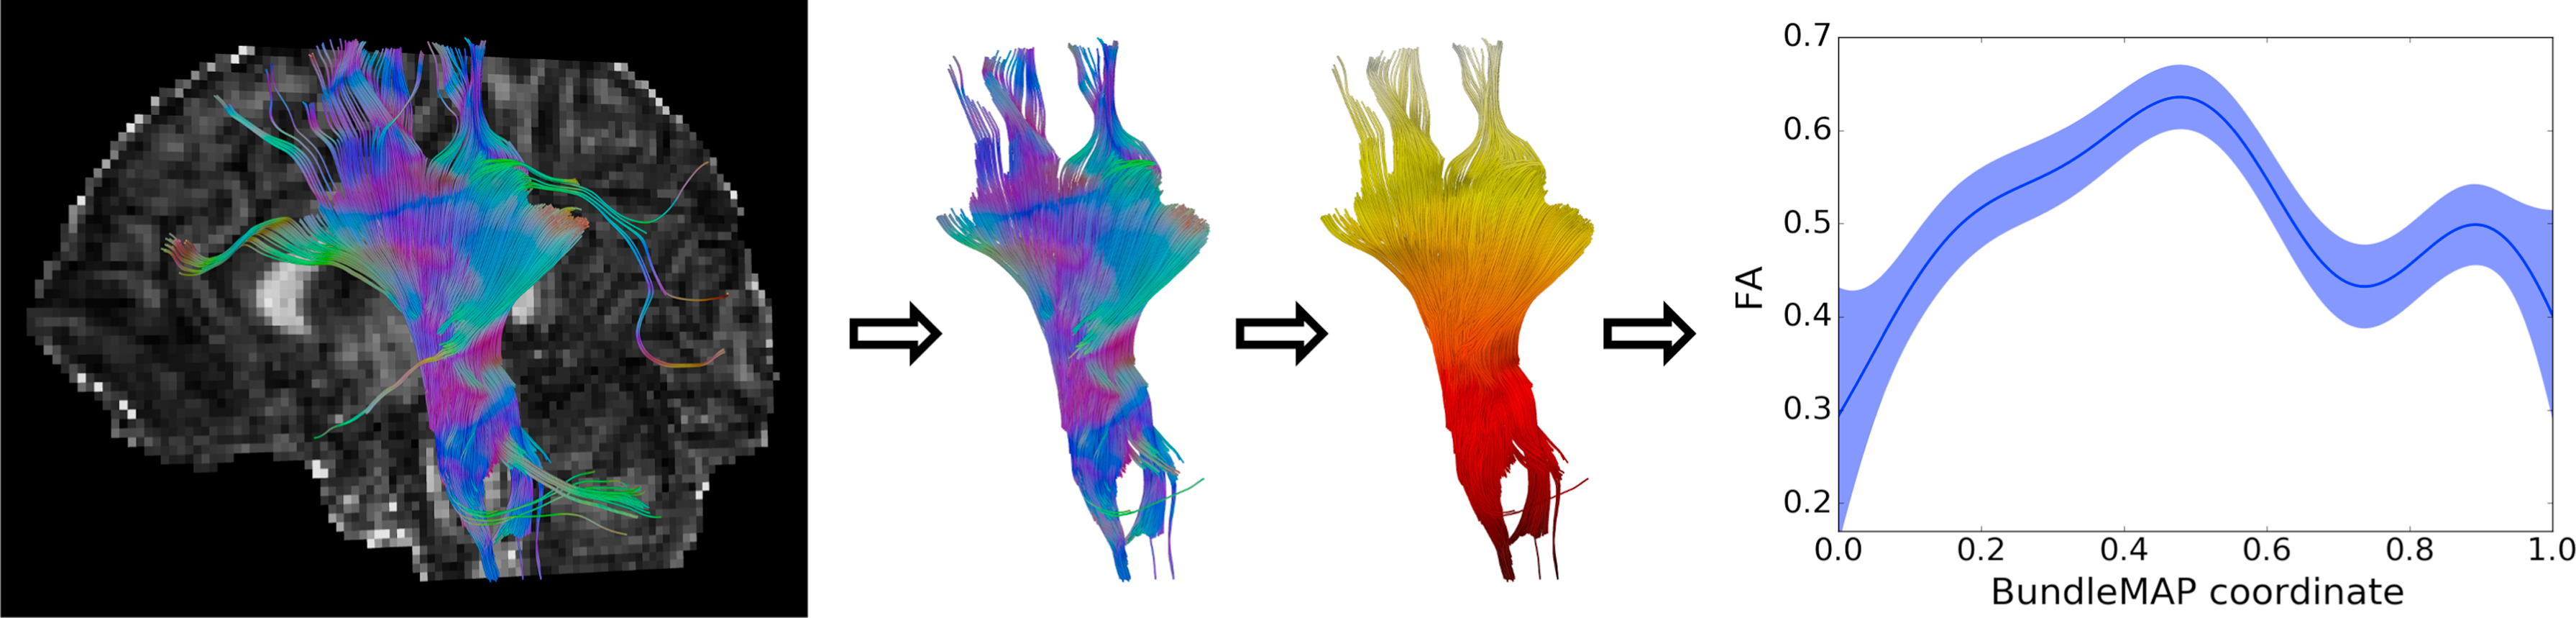
\includegraphics[width=14cm,height=14cm,keepaspectratio]{thesis_radomskyi/images/bundlemap_steps.jpg}
\caption{\textbf{BundleMAP Main Steps.} BundleMAP consists of four main steps: white matter fiber tractography, outlier removal, joint parametrization, and computation of spatially localised features along the BundleMAP coordinate \cite{Khatami2017BundleMap}}
\label{fig:bundlemap-steps}
\end{figure}

\subsubsection{Image preprocessing and tractography}
The first part of the BundleMAP processing pipeline consists of each subject's DWI data processing, extraction of diffusivity measures, and performing tractography for a set of predefined white matter tracts. These steps rely on principles adopted in VBA, namely analysis of subject population by performing registration towards a common template. In the case of BundleMAP, registration is performed by using Montreal Neurological Institute atlas, which represents an average, healthy human brain \cite{mniAtlasReference}. This introduces the presence of two different spaces -- one that is specific for the each of the subjects being processed (subject space), and the subject-agnostic MNI space. One of the advantages of using this approach, is the ability to predefine regions of interest in the space which is independent from the examined population, and then perform automatical mapping of these areas into the subject space.
The first data processing step within the pipeline is computation of fiber orientation distributions of the input dMRI images, using the spherical deconvolution algorithms \cite{dwi2fod2-csd, dwi2fod2-msmt-csd}, present within MRtrix \cite{mrtrixGeneral2019} and FSL \cite{fsl1, fsl2} software packages. This is followed by extraction of diffusion measures and using a registration algorithm to calculate two non-linear warp fields, which establish the spatial correspondence between the image and the MNI template. These steps produce all the data required for performing white matter tractography. Thereafter tractography is performed in the subject space using MRtrix \cite{mrtrixGeneral2019} implementation of the iFOD2 algorithm \cite{tckgen} for probabilistic streamlines tractography.

\subsubsection{Outlier removal}
Execution of voxelwise statistical analysis on a set of dMRI images is prone to multiple problems due to the imperfections of data and deficiency of registration and tracking algorithms \cite{voxelwiseImperfections}. In order to improve tracking data resulting from the first pipeline step, two strategies are implemented within the CoBundleMAP. The first one is based on the knowledge of the anatomy of human brain. Since the analysis is performed on a known set of white matter bundles, information about natural constraints of such bundles is applied to cut off any fibers that do not comply with predefined spacial thresholds. Afterwards all remaining fibers from all subjects are combined and processed using a one-class support vector machine (SVM), which identifies the smallest possible area in the input space that contains majority of the samples. Additionally, a parameter $\nu \in (0, 1]$ is specified, controlling the fraction of samples to be discarded \cite{Khatami2017BundleMap}.

\subsubsection{Manifold learning}
Computation of the joint fiber bundles parametrization across the whole examined population allows to perform a robust analysis by leveraging the inter-subject spatial correspondence of computed features within specific white matter tracts.
BundleMAP is based on the idea of representing individual white matter tracts as special cases of a generalized, abstract fiber bundle. Each fiber bundle core is thus regarded as a one-dimensional manifold, which then could be acquired through manifold learning techniques \cite{Khatami2017BundleMap}, such as ISOMAP \cite{isomapTenenbaum}. Fibers belonging to the same bundle are first warped to the MNI space using nonlinear transformations computed during image registration. In order to produce a \textit{joint} parametrization, ISOMAP algorithm needs to be applied to the accumulated data from the tracts of the whole population. Since the combined number of vertices across all subjects is too big for distance matrix calculation, BundleMAP first selects a set of representative streamlines, which will be used for manifold learning by performing \textit{k-means} clustering on tract fibers. Afterwards, vertices which belong to the selected streamlines are used for ISOMAP input. The values for the vertices that were excluded from the manifold computations, are interpolated as a weighted average of \textit{k} nearest vertices belonging to the representative fibres in MNI space \cite{Khatami2017BundleMap}. An example of the joint parametrization, produced by BundleMAP for the left corticospinal tract can be seen on Figure \ref{fig:bundlemap-parametrisation-results}.

\begin{figure}
\centering
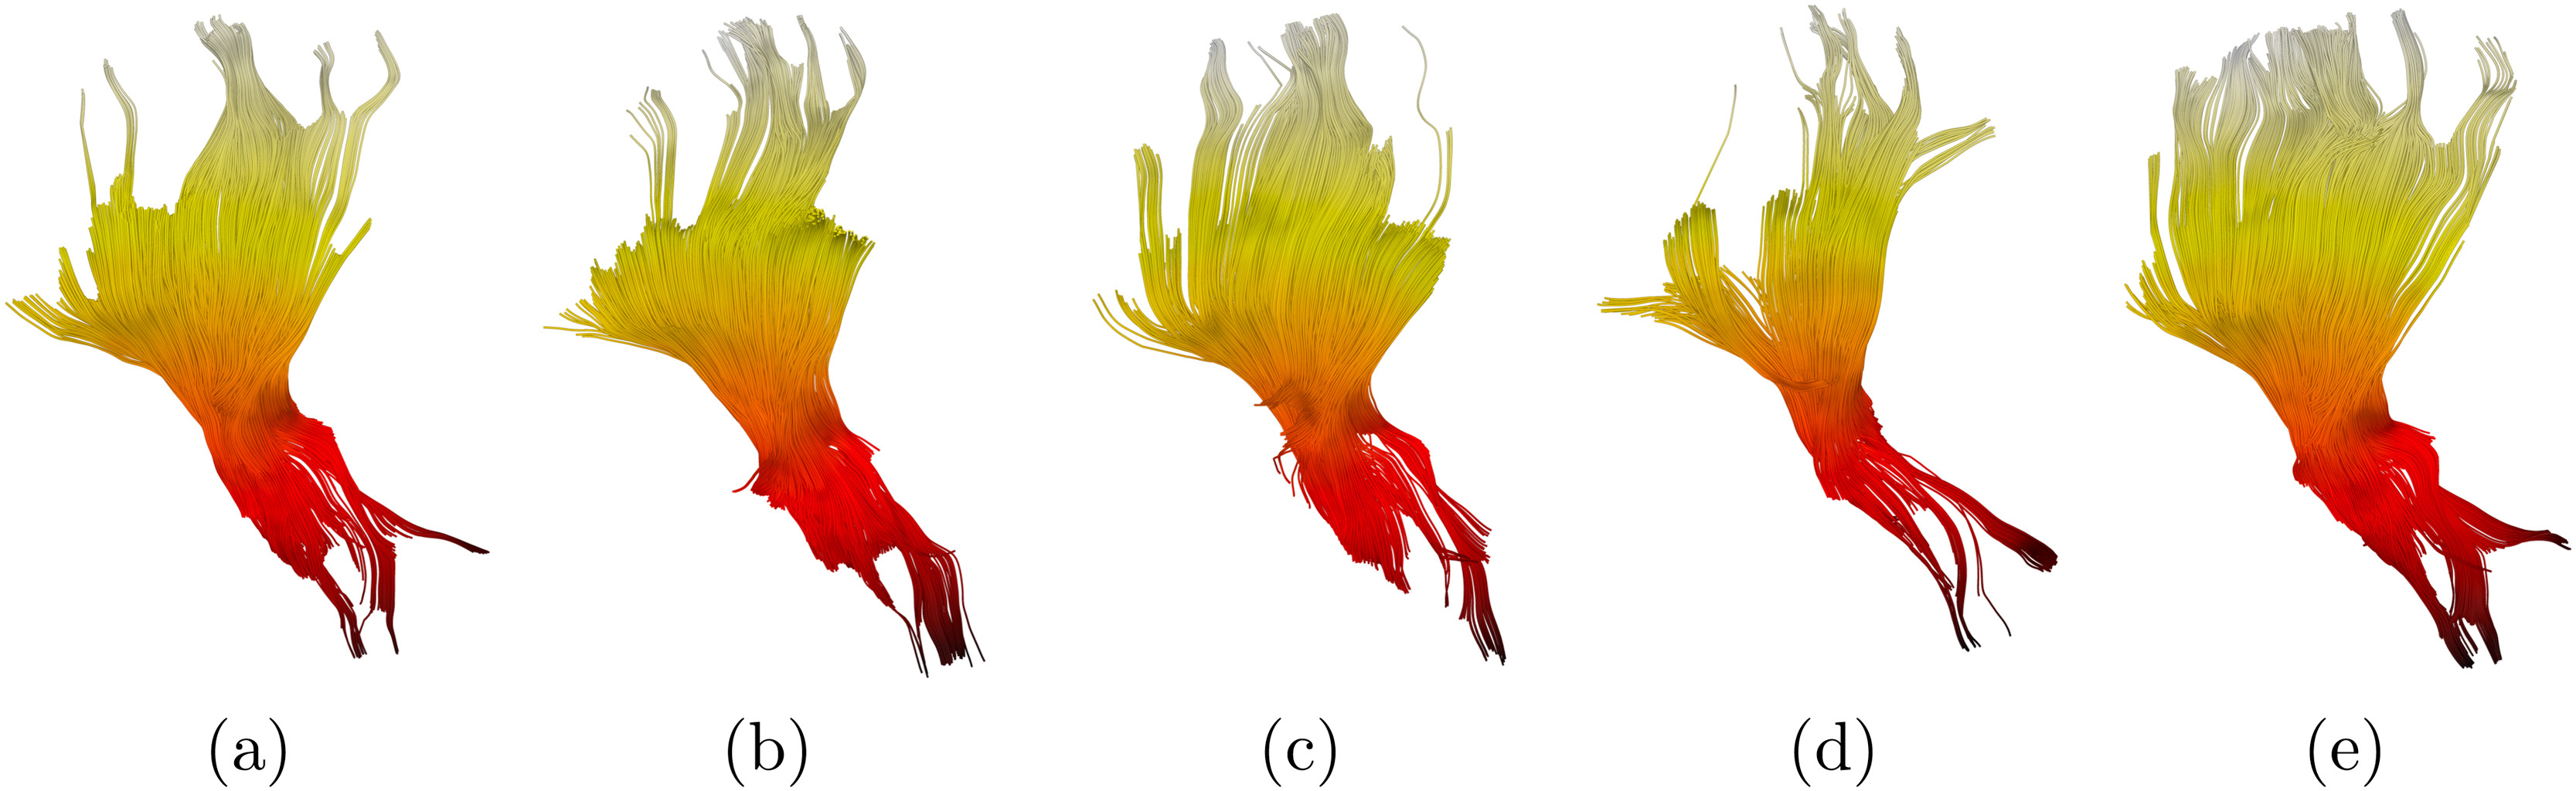
\includegraphics[width=14cm,height=14cm,keepaspectratio]{thesis_radomskyi/images/bundlemap-parametrisation-results.jpg}
\caption{\textbf{BundleMAP Joint Parametrization Results.} Image depicting results of joint parametrization of the left corticospinal tract, performed with BundleMAP. As can be seen, corresponding anatomical locations of the tract have matching colors, indicating correct parametrization \cite{Khatami2017BundleMap}}
\label{fig:bundlemap-parametrisation-results}
\end{figure}

\subsubsection{Feature extraction}
The streamlines and respective vertex values, produced via manifold learning, are represented as a function of ISOMAP coordinate, but since white matter bundles are of different size and proportions across the subjects, the range of ISOMAP coordinate is also varying within the population. In order to achieve a universal correspondence between the tracts, originating from distinct diffusion images, ISOMAP coordinate is normalised to the $[0,1)$ range. This allows to perform the analysis of extracted metrics along the reciprocal parts of the bundles, independent from dissimilarities of their initial size and form. BundleMAP pipeline produces feature vectors by partitioning the whole coordinate range into $n$ equal bins and assigning them an average of computed metrics values belonging to the corresponding segment of the tract.

\subsection{CoBundleMAP overview}
As mentioned before, CoBundleMAP is based on the same principles as the BundleMAP, but contains several important modifications that allow to considerably improve parameterization results. The most important changes are outlined in the corresponding source \cite{Khatami2019CoBundleMap}, in this subsection a short overview is given based on original paper and personal experience with the pipeline.

\subsubsection{Hemisphere correspondence}
One of the substantial differences of between CoBundleMAP and previous approach is computation of inter-hemisphere correlations between corresponding white matter bundles of individual subjects. This allows to achieve additional coherence between left and right parts of the same tract. This allows to significantly improve joint parametrization and observe additional asymmetries, leading to deeper insights about tissue structure and affected white matter bundles. To achieve this, CoBundleMAP computes registration of the points in the left tract to the corresponding points of the right tract by treating the vertices of the streamlines as point clouds and applying an iterative closest point approach \cite{Khatami2019CoBundleMap}. Consequently, the manifold learning is performed using streamlines from both hemispheres, producing an idealistic white matter bundle representation, expressing left and right tracts together. This is different from the approach used by BundleMAP, where each produced manifold was a manifestation of either right or left tract.

\subsubsection{Bundle parameterization}
Another prominent improvement of the new pipeline is the way how bundle processing and manifold learning are performed. CoBundleMAP is able to produce two-dimensional parameterization by setting the dimensionality of ISOMAP output. This allows to investigate changes of extracted diffusion parameters along two axis, distinguishing even more specific correlations. CoBundleMAP additionally improves the
mechanism of ISOMAP coordinate normalization. Instead of directly re-scaling produced result, the ranges of produced ISOMAP coordinates are first divided into discrete sections. Within these sections, number of contributing vertices is computed and compared against a predefined threshold, thus eliminating the sections that do not have enough support. This approach essentially trims the bundle ends, which tend to contain abnormally lower averaged metric values due to low sample count.


%\label{ch:background}

\end{document}